Internet of Things (IoT) refers to an idea that has been around since
1991\cite{iot_bonanza} that eventually all objects in the world will link into
one large network. Having all things linked in this way would require all
things to have microchips, or some sort of way to exchange and receive data.
This network of Things would result in astounding changes to all aspects of
life. Some examples include monitoring agriculture, parts to an airplane, and
controlling all aspects of a home. Multiple messaging protocols are
established with the goal of accomplishing IoT in the best possible fashion.
Protocols in development for IoT include the Extensible Messaging and Presence
Protocol (XMPP), Constrained Application Protocol (CoAP), and MQ Telemetry
Transport (MQTT)\cite{iot_linkedin}. In this paper, we observe and critique XMPP,
which contains protocol extensions specifically catered to IoT.

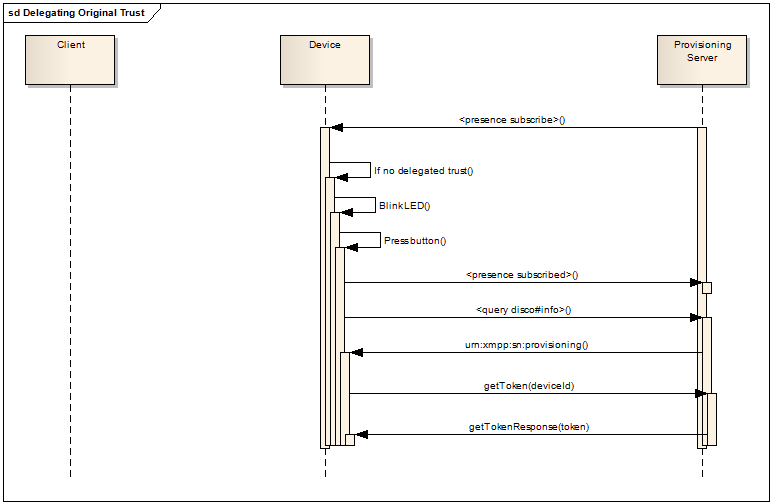
\includegraphics[scale=.25]{images/delegatingTrustSimpleNode}
